\documentclass[a4paper,ngerman]{scrartcl}

\usepackage{amsmath}
\usepackage{amsfonts}
\usepackage{amssymb}
\usepackage[utf8]{inputenc}
\usepackage{graphicx}
\usepackage[ngerman]{babel}
\usepackage{hyperref}
\usepackage{float}
\usepackage{caption}
\usepackage{subcaption}
\usepackage{multirow}  %for tables
\usepackage{icomma} % Handle german comma as decimal point in numbers
\usepackage{units,siunitx} % Write units with correct spacing
\usepackage{upgreek} % provide non-italic greek letters
\usepackage{url}
%\usepackage{subfig}

% Formatting of table & figure captions
\captionsetup{font={sf,footnotesize},labelfont=bf,textfont=sl,skip=6pt}
\setlength{\abovecaptionskip}{6pt}
\setlength{\belowcaptionskip}{0pt}

\title{Magnetisierung\\Versuchsvorbereitung}
\date{\today}
\author{Michel Rausch, Michael Eliachevitch}

\begin{document}

\maketitle
\tableofcontents
\newpage

\section{Einleitung}

%Versuchsbeschreibung:
%Es wird die Magnetisierung von Selten-Erd-Metallen (Tb, Gd)im Temperaturbereich T = 77 - 300 K bestimmt. 
%Dazu wird ein supraleitendes Quanteninterferometer (Superconducting Quantum-Interference Device, SQUID) aus einem Hochtemperatursupraleiter verwendet, das sich in einem Flüssigkstickstoff-gekühlten Dewar befindet.


\section{Theoretische Grundlagen}

\subsection{Supraleitung}


\subsection{Cooperpaare}


\subsection{Supraleiter im Magnetfeld}


\begin{figure}
\centering
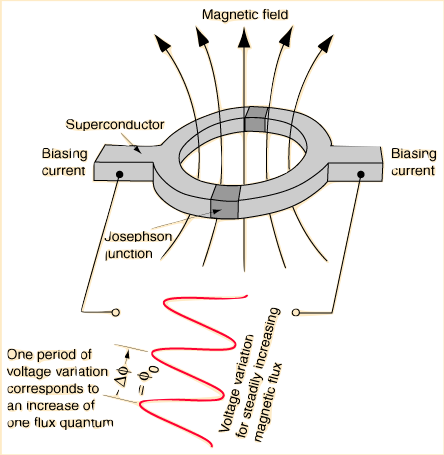
\includegraphics[width=0.7\textwidth]{abbildungen/squide.png}
\caption[Versuchsplatz]{\textbf{Flussfadengitter in einem Typ II-Supraleiter [\ref{ref:mappe}].}}
\label{fig:typII}
\end{figure}


\subsection{Meissner-Effekt}

\subsection{Josephson-Effekte}


\subsection{YBCO}

\subsubsection{Eigenschaften}

\subsubsection{Herstellung}


\section{Versuchsaufbau}

\subsection{SQUID}

\begin{figure}
\centering
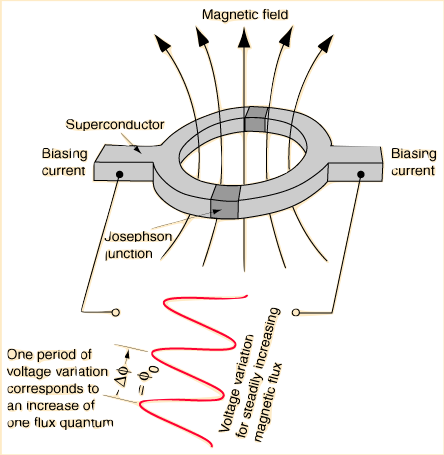
\includegraphics[width=0.7\textwidth]{abbildungen/squide.png}
\caption[Versuchsplatz]{\textbf{Aufbau eines SQUIDs [\ref{ref:wuppertal}].}}
\label{fig:squid_wuppertal}
\end{figure}

\subsubsection{Aufbau}

\subsubsection{Verhalten}

\subsection{Versuchsplatz}

\begin{figure}
\centering
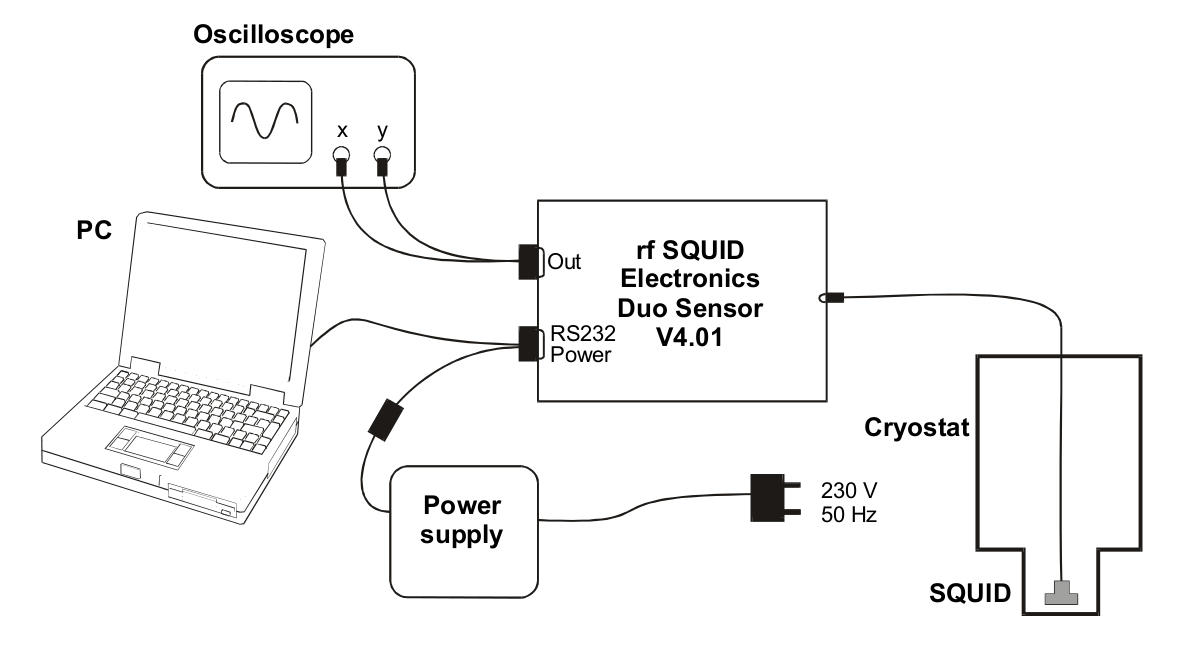
\includegraphics[width=0.7\textwidth]{abbildungen/aufbau_versuchsplatz.png}
\caption[Versuchsplatz]{\textbf{Aufbau des Versuchsplatz [\ref{ref:mappe}].}}
\label{fig:Versuchsplatz}
\end{figure}



\section{Versuchsdurchführung}


\section{Quellen}
\begin{enumerate}
\item Vorbereitungsmappe.\label{ref:mappe}
\item \url{http://hydrogen.physik.uni-wuppertal.de/hyperphysics/hyperphysics/hbase/solids/squid.html} ( 18.1.2015).\label{ref:wuppertal}
\end{enumerate}



\end{document}
